\documentclass{standalone}
\usepackage{tikz}
\begin{document}
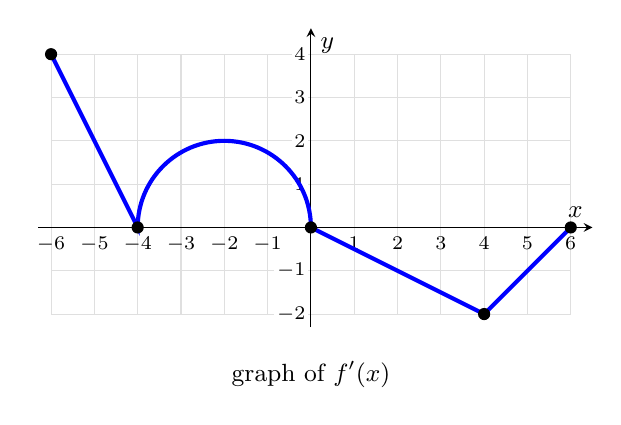
\begin{tikzpicture}[>=stealth, scale=0.55,
    curve/.style={blue, line width=1.5pt}]
  % Graph of f' on -6 <= x <= 6: three line segments and a semicircle
  %   segment (-6,4) -- (-4,0)
  %   upper semicircle centered at (-2,0), radius 2, from (-4,0) to (0,0)
  %   segment (0,0) -- (4,-2)
  %   segment (4,-2) -- (6,0)
  \def\xmin{-6}\def\xmax{6}
  \def\ymin{-2.3}\def\ymax{4.3}

  % Light grid
  \draw[gray!25] (\xmin,-2) grid[step=1] (\xmax,4);

  % Axes
  \draw[->] (\xmin-0.3,0) -- (\xmax+0.5,0) node[above left, font=\small] {$x$};
  \draw[->] (0,\ymin) -- (0,\ymax+0.3) node[below right, font=\small] {$y$};
  \foreach \x in {-6,-5,-4,-3,-2,-1,1,2,3,4,5,6}
    \node[below, font=\scriptsize] at (\x,0) {$\x$};
  \foreach \y in {-2,-1,1,2,3,4}
    \node[left, font=\scriptsize, fill=white, inner sep=1pt] at (-0.05,\y) {$\y$};

  % f'
  \draw[curve] (-6,4) -- (-4,0) arc[start angle=180, end angle=0, radius=2]
    -- (4,-2) -- (6,0);
  \foreach \p in {(-6,4), (-4,0), (0,0), (4,-2), (6,0)}
    \fill \p circle (4pt);

  % Caption
  \node[font=\small] at (0,-3.4) {graph of $f'(x)$};
\end{tikzpicture}
\end{document}
